\documentclass[11pt,a4paper]{article}

%% ---- Package imports ----------------------------------------
\usepackage[utf8]{inputenc}
\usepackage[margin=1in]{geometry}
\usepackage{amsmath,amssymb,amsfonts}
\usepackage{booktabs}
\usepackage{xcolor}
\usepackage{graphicx}
\usepackage{hyperref}
\usepackage{microtype}
\usepackage{enumitem}
\usepackage{array}

%% ---- TikZ Setup ---------------------------------------------
\usepackage{tikz}
\usetikzlibrary{shapes.geometric, arrows.meta, positioning, calc}

%% ---- Hyperref Config ----------------------------------------
\hypersetup{
  colorlinks = true,
  linkcolor  = blue!60!black,
  citecolor  = blue!60!black,
  urlcolor   = blue!60!black
}

\begin{document}

%% ============================================================================
%%  INSTITUTIONAL HEADER & TITLE BLOCK
%% ============================================================================
\begin{center}
  {\large\textbf{RV COLLEGE OF ENGINEERING, BENGALURU - 560059}} \\
  {\small\textit{(An Autonomous Institution Affiliated to VTU, Belagavi)}} \\
  {\small\textbf{DEPARTMENT OF COMPUTER SCIENCE AND ENGINEERING}} \\
  \vspace{0.4cm}
  {\large\textbf{CONCEPT PROPOSAL DOCUMENT}} \\
  {\small\textit{Internal Departmental/Institutional Review Submission (Academic Year 2024--25)}} \\
  \vspace{0.8cm}
  
  \rule{\textwidth}{1pt} \\
  \vspace{0.3cm}
  {\Large\textbf{EpiSentinel: AI-Powered Dengue Outbreak Forecasting\\ and Decision Support for Karnataka}} \\
  \vspace{0.3cm}
  \rule{\textwidth}{1pt} \\
  \vspace{0.6cm}
\end{center}

\noindent
\begin{tabular}{@{}ll}
  \textbf{Submitted By:} & \textbf{Project Guide:} \\
  Ekansh Nandan Sharma (1RV23CS046) & Prof. Saraswathi Govind Datar \\
  GN Disha (1RV23CS0\_\_) & Assistant Professor \\
  Ishan Mahajan (1RV23CS0\_\_) & Department of Computer Science Engineering \\
  Bachelor of Engineering, CSE & RV College of Engineering \\
  RV College of Engineering, Bengaluru & Email: \texttt{saraswathigd@rvce.edu.in} \\
\end{tabular}

\vspace{0.8cm}

%% ============================================================================
\section{Problem Statement}
\label{sec:problem}
%% ============================================================================
Dengue fever is a severe and rapidly growing vector-borne public health challenge in Karnataka. Over the past several years, the state has experienced a marked, year-on-year increase in both dengue morbidity and spatial spread. The disease is endemic across urban and rural districts alike, placing immense stress on regional healthcare systems during peak transmission seasons.

The fundamental bottleneck in managing dengue is that the current government surveillance infrastructure, primarily anchored by the Integrated Disease Surveillance Programme, is structurally reactive. The system relies on passive reporting, where case records are collected from clinics, aggregated at the district level, and sent to state registries. This reporting pipeline introduces a lag of two to three weeks. Consequently, by the time public health officers at the Directorate of Health and Family Services receive an official outbreak alert, the transmission wave has already peaked in the community. As a result, vector control measures (such as larvicide spraying and fogging) and medical resources (such as intravenous fluids and blood bank supplies) are deployed too late to prevent preventable infections or reduce hospitalization rates.

Fortunately, there is a clear biological window of predictability that can be exploited. A dengue transmission cycle is triggered by environmental shifts. Heavy rainfall, coupled with specific temperature and humidity ranges, creates ideal breeding environments for \textit{Aedes aegypti} mosquitoes. This is followed by a fixed biological timeline: mosquito breeding and larval development take seven to ten days, the viral incubation inside the mosquito takes another eight to fourteen days, and the incubation period in humans takes four to seven days. In total, environmental triggers occur approximately three to four weeks before clinical cases actually manifest in hospital records. Furthermore, once an outbreak starts, the ongoing case counts encode a powerful statistical momentum: active infections in a neighborhood directly predict new cases in the subsequent week.

Currently, health officers in Karnataka lack an integrated tool that translates historical and real-time environmental data into early warnings. Existing research models focus on academic predictions without providing local explanations or practical recommendations. Health administrators need a unified dashboard that delivers an early warning alert, explains the underlying drivers of the current risk, and provides a clear, official standard operating procedure advisory in a single, accessible interface.

\newpage

%% ============================================================================
\section{Proposed Solution}
\label{sec:solution}
%% ============================================================================
EpiSentinel is an end-to-end, web-based artificial intelligence dashboard designed to predict district-level dengue outbreaks in Karnataka seven days in advance. The system is built to bridge the gap between complex machine learning and the operational needs of non-technical public health administrators, providing them with early, actionable, and explainable foresight.

The core of EpiSentinel is its prediction engine, which analyzes two distinct types of signals simultaneously. First, it tracks local epidemiological momentum by looking at how case counts have trended over the previous four weeks (the primary predictor). Second, it monitors localized environmental variables, including temperature, relative humidity, and cumulative rainfall. By combining these signals, the system predicts whether a district's dengue case count in the upcoming week will exceed its historical threshold, signaling an impending outbreak.

EpiSentinel generates predictions for all districts in Karnataka. These risk levels are visualised on an interactive, color-coded map categorized into three operational tiers: Low Risk (green), High Risk (orange), and Critical Risk (red). This enables state-level health directors to assess the entire state's vulnerability at a single glance.

Crucially, the dashboard does not simply output a black-box percentage. It provides a transparent explanation of why a district's risk has shifted. For example, if a district is flagged as Critical, the interface displays a clear, plain-language summary such as: ``Risk is critical due to a sustained upward trend in local case counts over the past three weeks, modulated by a significant spike in rainfall fourteen days ago.''

To convert warnings into direct public health action, EpiSentinel includes an AI-powered advisory assistant named Sentinel AI. When a district is flagged as High or Critical Risk, Sentinel AI retrieves Karnataka's official government standard operating procedures for vector-borne disease control. It then automatically generates a structured, step-by-step action plan tailored to that specific district's risk level. This action plan outlines specific tasks for the current week, including larviciding protocols, hospital bed allocations, and public awareness campaigns, ensuring that health officers can transition immediately from observation to intervention.

\begin{figure}[htbp]
  \centering
  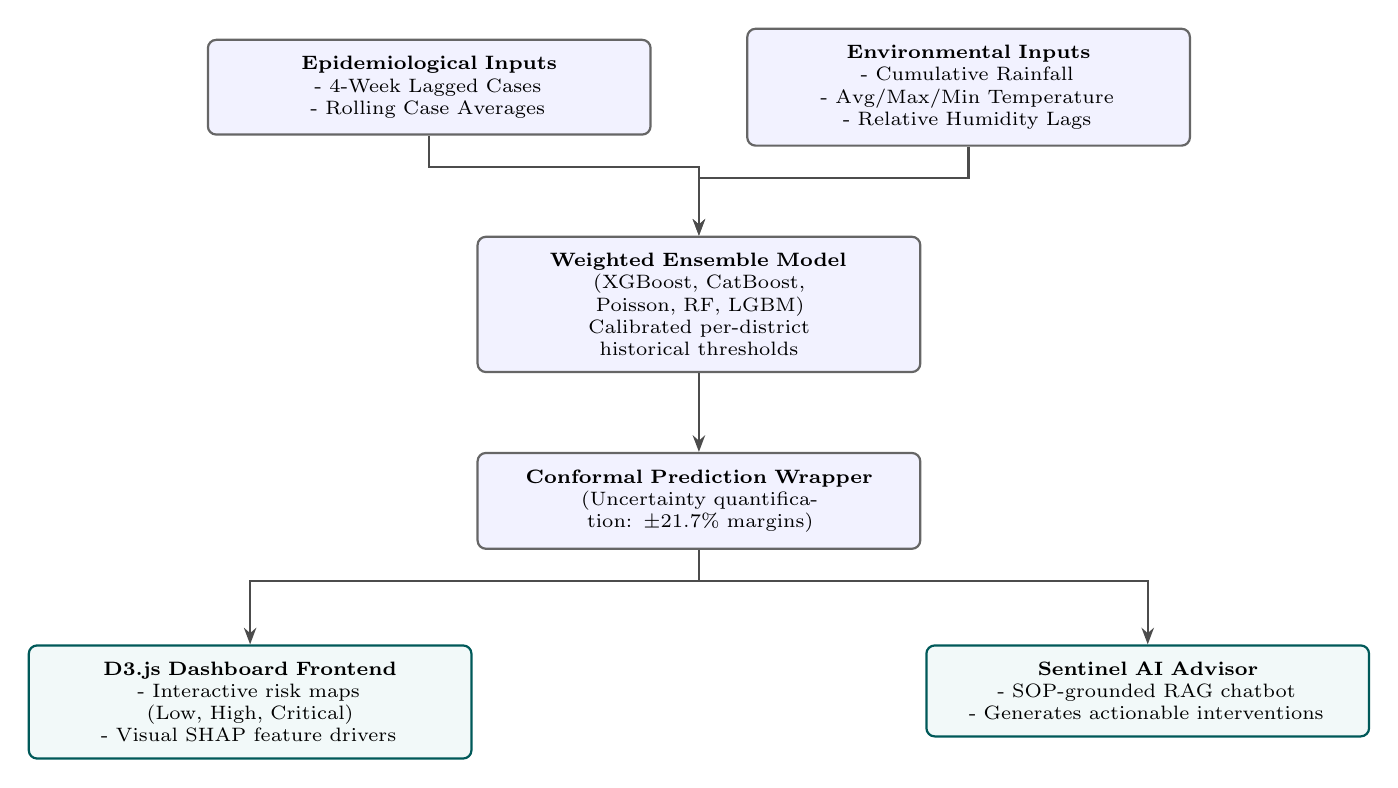
\begin{tikzpicture}[
    node distance=1.0cm and 1.2cm,
    box/.style={
      rectangle, rounded corners=3pt,
      draw=black!60, thick,
      fill=blue!5, 
      text width=5.2cm, align=center,
      font=\scriptsize, inner sep=6pt
    },
    gbox/.style={
      rectangle, rounded corners=3pt,
      draw=teal!70!black, thick,
      fill=teal!5, 
      text width=5.2cm, align=center,
      font=\scriptsize, inner sep=6pt
    },
    arr/.style={-{Stealth[length=6pt]}, thick, color=black!70}
  ]
    \node[box] (input1) {
      \textbf{Epidemiological Inputs}\\
      - 4-Week Lagged Cases\\
      - Rolling Case Averages
    };
    \node[box, right=of input1] (input2) {
      \textbf{Environmental Inputs}\\
      - Cumulative Rainfall\\
      - Avg/Max/Min Temperature\\
      - Relative Humidity Lags
    };
    
    \node[box, below=1.2cm of $(input1.south)!0.5!(input2.south)$] (model) {
      \textbf{Weighted Ensemble Model}\\
      (XGBoost, CatBoost, Poisson, RF, LGBM)\\
      Calibrated per-district historical thresholds
    };
    
    \node[box, below=of model] (conformal) {
      \textbf{Conformal Prediction Wrapper}\\
      (Uncertainty quantification: $\pm 21.7\%$ margins)
    };
    
    \node[gbox, below left=1.2cm and 0.05cm of conformal] (map) {
      \textbf{D3.js Dashboard Frontend}\\
      - Interactive risk maps (Low, High, Critical)\\
      - Visual SHAP feature drivers
    };
    
    \node[gbox, below right=1.2cm and 0.05cm of conformal] (chatbot) {
      \textbf{Sentinel AI Advisor}\\
      - SOP-grounded RAG chatbot\\
      - Generates actionable interventions
    };
    
    \draw[arr] (input1.south) -- +(0,-0.4) -| (model.north);
    \draw[arr] (input2.south) -- +(0,-0.4) -| (model.north);
    \draw[arr] (model) -- (conformal);
    \draw[arr] (conformal.south) -- +(0,-0.4) -| (map.north);
    \draw[arr] (conformal.south) -- +(0,-0.4) -| (chatbot.north);
  \end{tikzpicture}
  \caption{EpiSentinel end-to-end decision-support flow diagram.}
  \label{fig:flowchart}
\end{figure}

\newpage

%% ============================================================================
\section{Key Innovations}
\label{sec:innovations}
%% ============================================================================
\begin{enumerate}[label=\arabic*., leftmargin=*]
  \item \textbf{Primary reliance on recent case trends:} The framework prioritizes localized, short-term epidemiological case momentum over weather variables, as active transmission indicators carry significantly higher predictive power at a seven-day forecast horizon.
  \item \textbf{District-level custom calibration:} Outbreak thresholds are calculated based on each district's unique historical data rather than using a uniform statewide average, ensuring that small districts like Kodagu and large urban hubs like Bengaluru Urban are evaluated against their own historical norms.
  \item \textbf{Rigorous data-leakage auditing:} The machine learning pipeline includes a three-stage audit to prevent the models from memorizing static geographical features or historical baseline statistics, guaranteeing that the system learns real, generative epidemiological patterns.
  \item \textbf{Principled confidence intervals:} Every risk prediction is accompanied by a rigorous mathematical confidence range (e.g., ``84\% risk, confidence range 71\% to 93\%''), giving administrators a clear metric of how certain the model is before they commit financial or human resources.
  \item \textbf{Strictly-grounded advisory generation:} The Sentinel AI chatbot is built using an information-lookup framework restricted to official Karnataka health protocols, completely preventing the AI from fabricating advisory information or generating unverified guidelines.
\end{enumerate}

\vspace{0.4cm}

%% ============================================================================
\section{Technical Approach}
\label{sec:technical}
%% ============================================================================
The technical architecture of EpiSentinel consists of a modular machine learning pipeline linked to a web application.

The core forecasting engine utilizes a Weighted Ensemble model that combines five complementary algorithms: XGBoost, CatBoost, LightGBM, Random Forest, and Poisson Regression. The sub-models were trained on historical weekly district-level panel data spanning from 2017 to 2021. Testing and final evaluation were performed on a completely held-out temporal test set consisting of the entire 2023 calendar year to simulate real-world operational performance.

The model demonstrates high reliability, capturing 85.6\% of actual historical outbreaks (Recall = 0.856), which is critical for minimizing dangerous false negatives. It achieves an overall balance of 0.720 (F1-Score) and a strong classification area of 0.821 (ROC-AUC) on the 2023 test set.

Explainability is achieved through SHAP (SHapley Additive exPlanations), a game-theoretic method that calculates the exact contribution of each feature to a given prediction. The system automatically extracts the single most influential driver for each inference and translates it into a plain-text explanation displayed on the map.

The Sentinel AI assistant is implemented using Retrieval-Augmented Generation. Rather than allowing the underlying language model to generate answers from its general training data, the chatbot uses a vector database containing official vector-control and clinical management standard operating procedures. When a user asks for an advisory plan, the system retrieves the specific sections of the SOP relevant to the district's current risk tier and uses them as the sole source material for the advice, ensuring complete alignment with official protocols.

The system is deployed as a lightweight web application. The backend is powered by FastAPI (Python) to serve predictions, SHAP explanations, and RAG chatbot queries. The frontend is built using HTML, CSS, and D3.js to render the interactive district-level map, providing a smooth, responsive, and secure experience.

\begin{table}[htbp]
  \caption{Weighted Ensemble Performance (2023 Test Set)}
  \label{tab:metrics}
  \centering
  \begin{tabular}{lcl}
    \toprule
    \textbf{Evaluation Metric} & \textbf{Value} & \textbf{Operational Interpretation} \\
    \midrule
    Outbreak Recall Rate (Recall) & 85.6\% & Captures 85.6\% of actual outbreak events \\
    Balanced F1-Score (F1)        & 0.720  & Strong harmonic mean of Precision and Recall \\
    ROC-AUC Area                  & 0.821  & High reliability in risk categorization ranking \\
    Conformal Margin Width ($\hat{q}$) & $\pm 21.7\%$ & 90\% confidence range for risk points \\
    \bottomrule
  \end{tabular}
\end{table}

\begin{figure}[htbp]
  \centering
  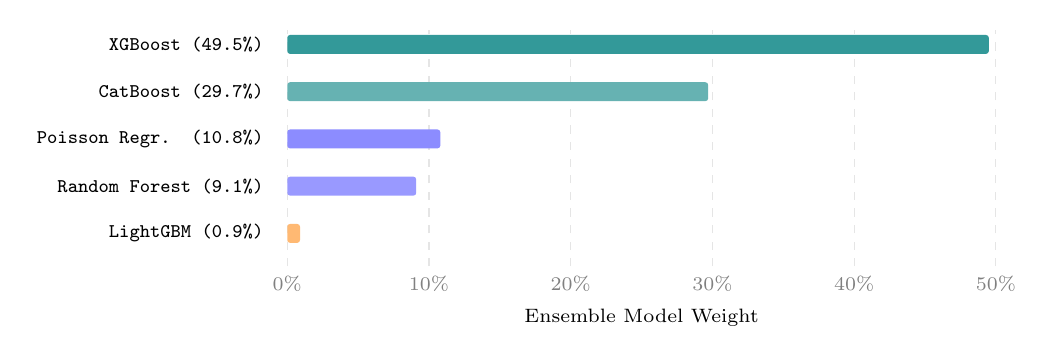
\begin{tikzpicture}[yscale=0.6, xscale=0.18]
    % Draw grid lines
    \foreach \x in {0, 10, 20, 30, 40, 50} {
      \draw[gray!20, dashed] (\x, -0.5) -- (\x, 4.5);
      \node[below, font=\scriptsize, text=gray] at (\x, -0.5) {\x\%};
    }
    
    % XGBoost: 49.5%
    \fill[teal!80, rounded corners=1pt] (0, 4) rectangle (49.5, 4.4);
    \node[anchor=east, font=\scriptsize\ttfamily] at (-1, 4.2) {XGBoost (49.5\%)};
    
    % CatBoost: 29.7%
    \fill[teal!60, rounded corners=1pt] (0, 3) rectangle (29.7, 3.4);
    \node[anchor=east, font=\scriptsize\ttfamily] at (-1, 3.2) {CatBoost (29.7\%)};
    
    % Poisson: 10.8%
    \fill[blue!45, rounded corners=1pt] (0, 2) rectangle (10.8, 2.4);
    \node[anchor=east, font=\scriptsize\ttfamily] at (-1, 2.2) {Poisson Regr. (10.8\%)};
    
    % Random Forest: 9.1%
    \fill[blue!40, rounded corners=1pt] (0, 1) rectangle (9.1, 1.4);
    \node[anchor=east, font=\scriptsize\ttfamily] at (-1, 1.2) {Random Forest (9.1\%)};
    
    % LightGBM: 0.9%
    \fill[orange!55, rounded corners=1pt] (0, 0) rectangle (0.9, 0.4);
    \node[anchor=east, font=\scriptsize\ttfamily] at (-1, 0.2) {LightGBM (0.9\%)};
    
    % X-axis label
    \node[below, font=\scriptsize] at (25, -1.2) {Ensemble Model Weight};
  \end{tikzpicture}
  \caption{Weighted ensemble model composition and contributions.}
  \label{fig:weights}
\end{figure}

\newpage

%% ============================================================================
\section{Relevance and Impact}
\label{sec:relevance}
%% ============================================================================
Karnataka is home to approximately 67 million people, and dengue is endemic across most of its districts. During transmission spikes, public hospitals experience surges in admissions, blood supply shortages, and diagnostic delays, which increase morbidity and cause preventable deaths.

Even a single week of advance warning provides public health officers with enough time to take preventative action. Within seven days, local municipalities can deploy targeted larvicide treatment, schedule space-spraying (fogging) in high-risk clusters, pre-position platelet counts and IV fluids in primary health centers, and alert local medical staff. These early, low-cost activities are significantly more effective at reducing transmission than late-stage emergency responses. Furthermore, this proactive model aligns directly with India's National Vector Borne Disease Control Programme guidelines, which emphasize community-level source reduction and early diagnosis.

It is important to note that ARTPARK at the Indian Institute of Science, Bengaluru, has developed an operational outbreak tracking system called PRISM-H for Karnataka. EpiSentinel is an independent student research project that explores complementary innovations. Specifically, EpiSentinel focuses on local model explainability (SHAP), principled uncertainty quantification (conformal prediction), and automated, SOP-grounded AI-driven decision support (Retrieval-Augmented Generation advisories)---methodologies that are not present in current operational frameworks.

This work is currently being compiled into a full, publication-ready LaTeX research paper. The manuscript will be submitted to a peer-reviewed IEEE journal to share these findings with the wider scientific community.

\vspace{0.4cm}

%% ============================================================================
\section{Project Status}
\label{sec:status}
%% ============================================================================
The EpiSentinel project has completed its core development phases. The weighted machine learning ensemble model is fully trained, optimized, and saved. The FastAPI backend and interactive D3.js web frontend are complete and fully operational locally, displaying predictions, confidence ranges, and SHAP-based explanations. The retrieval-augmented advisory chatbot is fully integrated and tested, producing actions strictly grounded in the vector-stored standard operating procedures. The accompanying research paper is currently in its final drafting stage, formatted to IEEE standards, and is undergoing internal review prior to formal submission.

\vspace{0.4cm}

%% ============================================================================
\section{Conclusion}
\label{sec:conclusion}
%% ============================================================================
EpiSentinel represents a significant step forward in dengue prevention by moving public health decision-making from a reactive to a proactive model. By combining robust ensemble forecasting with explainable AI and automated, protocol-grounded advisory generation, the system provides health officers with a clear, actionable tool for early intervention. Future work will explore integrating live automated API weather feeds and incorporating spatial correlations across neighboring districts to further refine prediction accuracy.

\end{document}
